\documentclass[a4paper,10pt]{report}

\usepackage[left=3cm,right=3cm,top=2cm,bottom=3cm]{geometry}
\usepackage{palatino}
\usepackage{graphicx}
\usepackage{amssymb}
\usepackage{amsmath}

% Title Page
\title{PHYS341 Design Experiment \\ AM Radio}
\author{David Harris \\ 300069566}


\begin{document}

\maketitle
\tableofcontents
\begin{abstract}
  The design task was to build an AM radio out of discrete components.
  This task was divided into five sections.  In order, these are the
  emitter follower, common base, rectifier circuit, OP amp circuit and
  power amplifier.  The emitter follower acts as a current buffer with
  it's high input and low output impedance.  This is then connected to
  a pair of common base amplifiers, giving a total voltage gain of
  approximately 1000.  This is then connected to a rectifier which
  separates the carrier and the data signals.  The sound waves are
  then passed through a op amp, which amplifies the signal so it able
  to be heard.  The final stage of the circuit is a power amp that
  gives enough power to drive the speaker.

  I have tested each section of the circuit individually when
  constructing the radio, making sure that each works the way it
  should.  However, when putting the circuit together as a whole, no
  sound is heard.  This could be a wide range of things, which I
  detail in the Problems section.
\end{abstract}

\chapter{Introduction}
The radio was built in five sections, each performing one task to
enable to whole system to function.  The demodulator, or 'tuning
circuit' was given to us as plug-in.  This consisted of an inductor
and a variable resistor that actually tuned in to the radio
frequencies.  The antenna was attached to this.  This then connected
to the emitter follower (or common collector). This boosts the current
of the input signal, while giving no voltage gain.  This sets the
impedance of the circuit, as the impedances between the components
must match, otherwise each section forms a voltage divider.
Therefore, the output impedance of the emitter follower must be the
same as the input impedance of the common base amplifier.  The common
base amplifier has a voltage gain of about 1000.  To do keep the
circuit stable, this has been done in two separate amplifiers with a
gain of 500 each.  Having a gain of 1000 made some ringing in the
circuit, and some complex negative feedback would have been needed to
combat it.  Now with both the current and voltage increased, the
signal was passed through a rectifier circuit.  This separated the
actual data signal, from the carrier signal.  This consisted of a
capacitor and resistor in series.  The values of these were chosen so
as to make the time constant between the period of the AM radio signal
and the spoken voice.  The data signal is then amplified by an op amp
with a gain of about 10.  This gives the signal enough amplification
so it can be hard out of the speaker.  The last stage is a Power amp,
which increases the current, so the speakers can be driven.
\pagebreak

\chapter{Description of Design Task}
The overall block diagram of the radio is shown below.  All the parts
were constructed and tested individually before incorporating it into
the rest of the circuit.

\begin{figure}[htb]
  \centering
  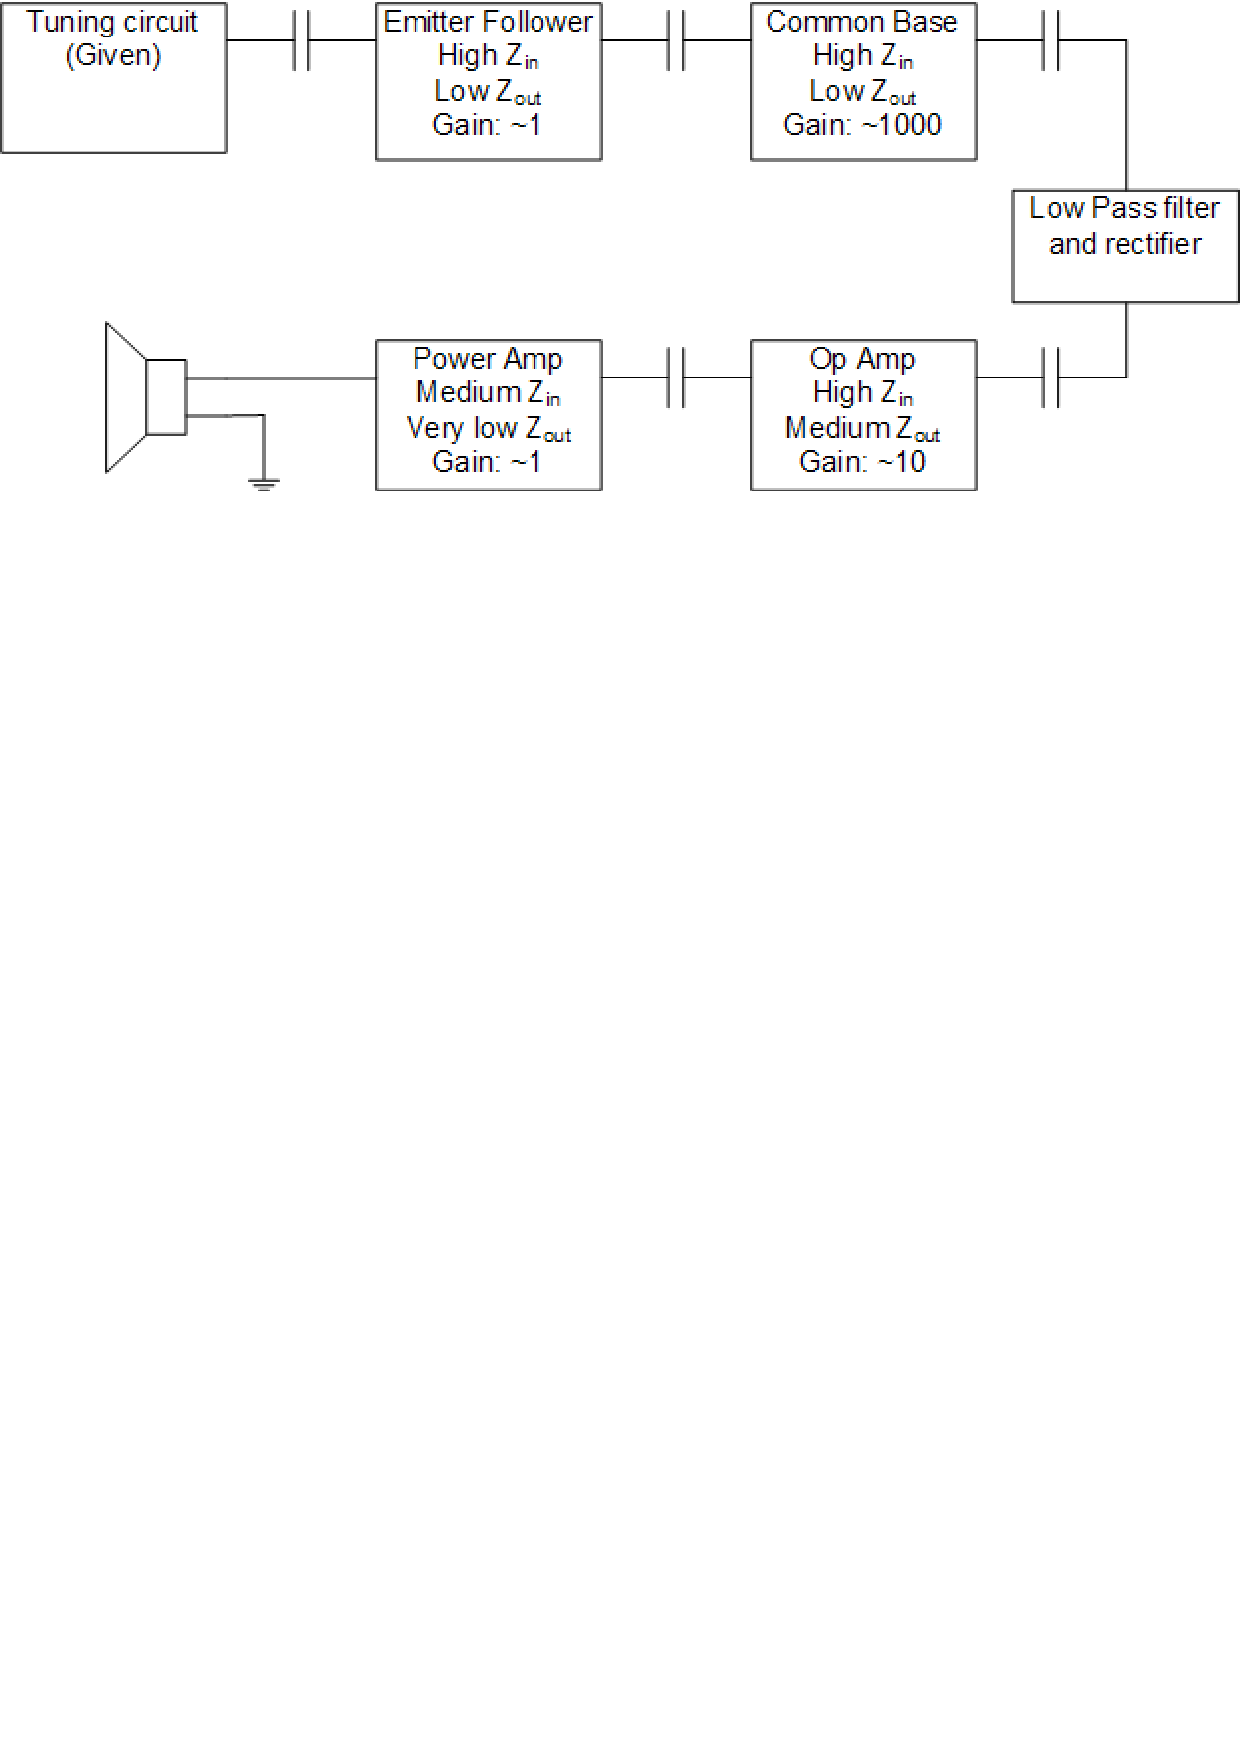
\includegraphics[scale=0.5]{Block-diagram}
  \caption{Block Diagram of the radio}
\end{figure}

The emitter follower (or common collector) was designed so as to have
an input impedance of about 100k? and an output impedance of less than
1k? and a bandwidth of 500kHz to 1.6MHz.  The advantage of an emitter
follower is that it has a low output resistance and high input
resistance, which means that it has a large current gain.  It is the
first amplification stage because once the current is increased, the
voltage can next be increased in the next stage, to give a larger
input signal.  For the details of how the emitter follower was biased,
see the appendices.  The next stage was the common base, which acted
as an RF amplifier.  As the current was now at a suitable level, the
voltage could not be amplified.  The desired gain was about 1000,
without the transistor going into saturation.  The main
characteristics of the common base are a very low input resistance,
relatively high input resistance and a large gain.  The circuit
diagram of the emitter follower and common base are shown below.

\begin{figure}[h]
  \centering
  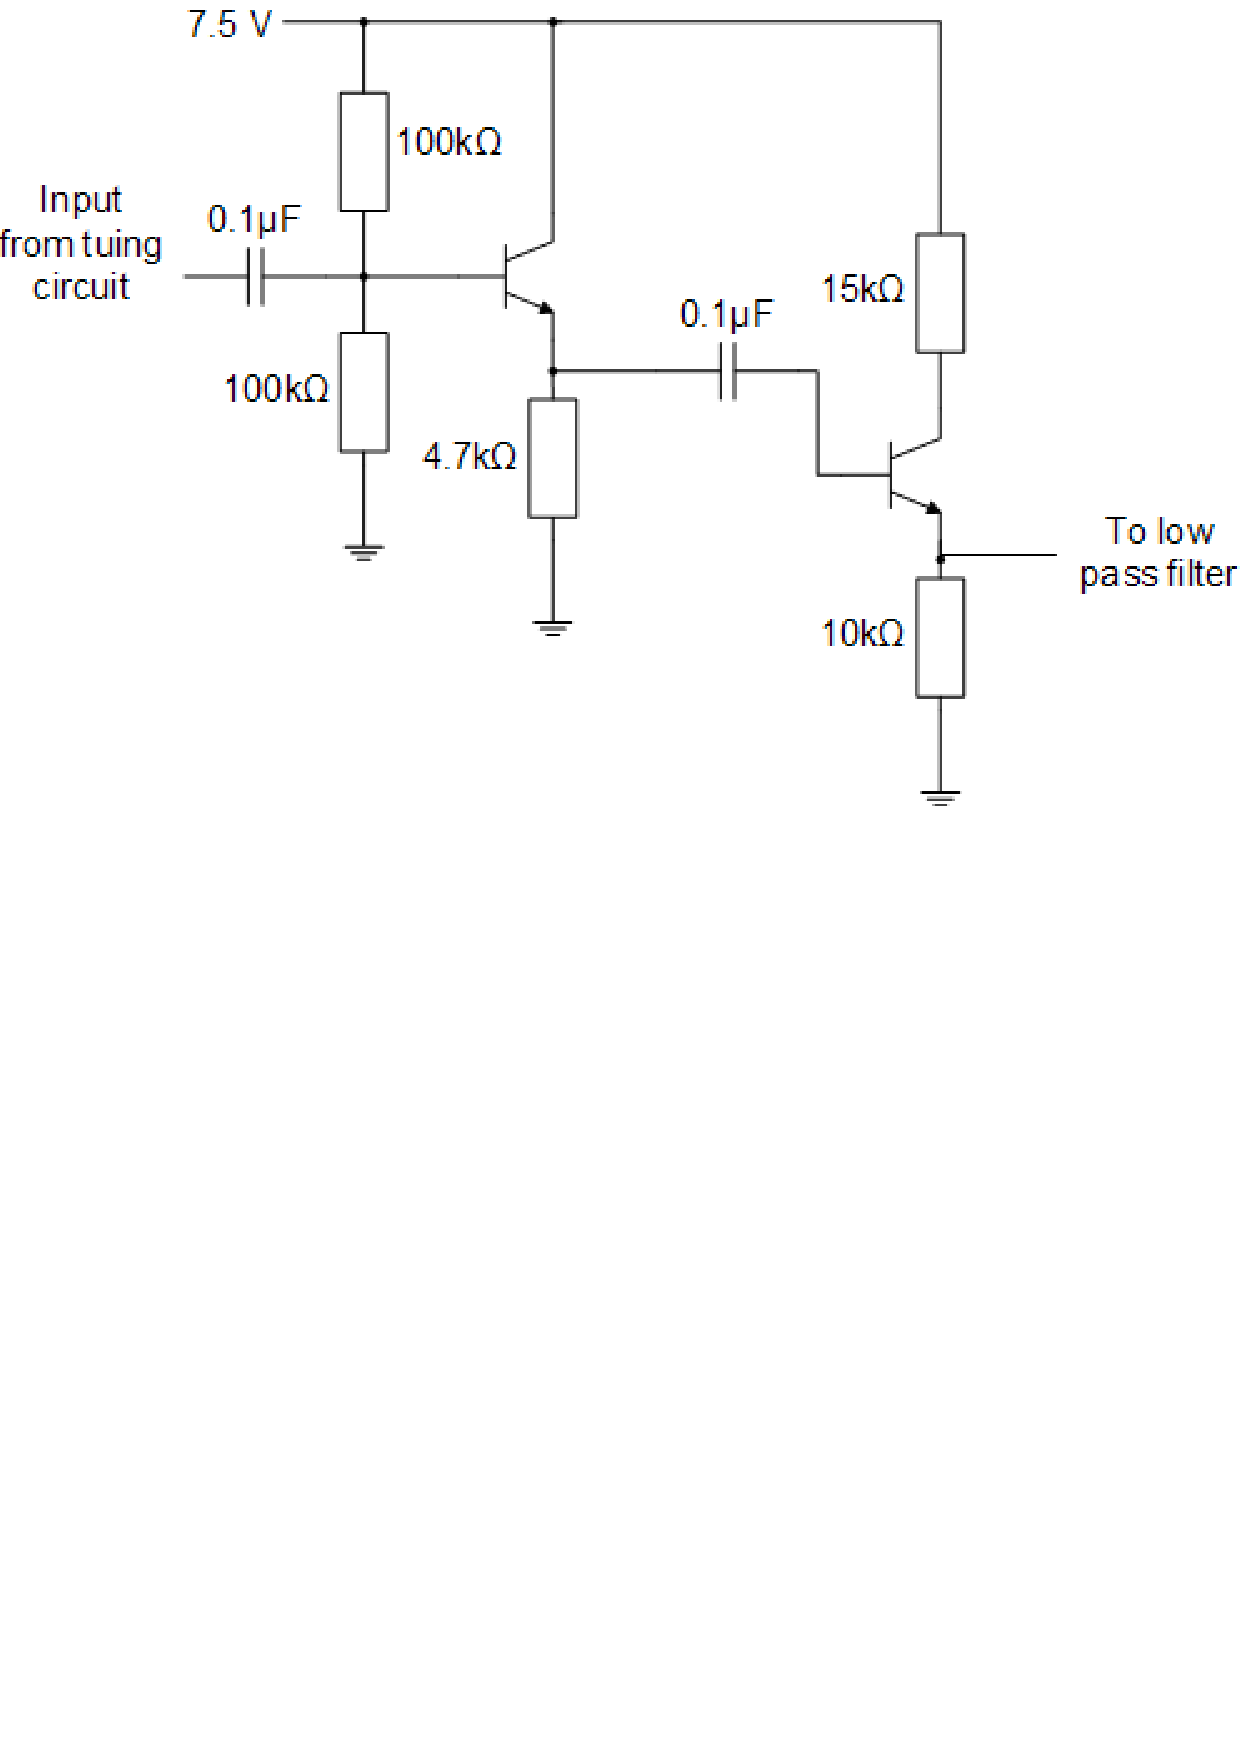
\includegraphics[scale=0.45]{Emitter-follower}
  \caption{Emitter Follower and Common Base Configuration}
\end{figure}

The signal then went through a rectifier and a low-pass filter.  The
rectifier blocked the negative part of the incoming sinusoidal wave,
and the low-pass filter separated the signal from the carrier wave,
and allowed the signal to pass through.  The values of the resistor
and capacitor had to be chosen carefully to ensure they allowed the AM
band (500kHz to 1.6MHz) was not passed through, but the voice (20Hz to
20kHz) was.  The components formed a RC circuit with a time constant
$\tau$ = RC.  The configuration is shown below.

\begin{figure}[htb]
  \centering
  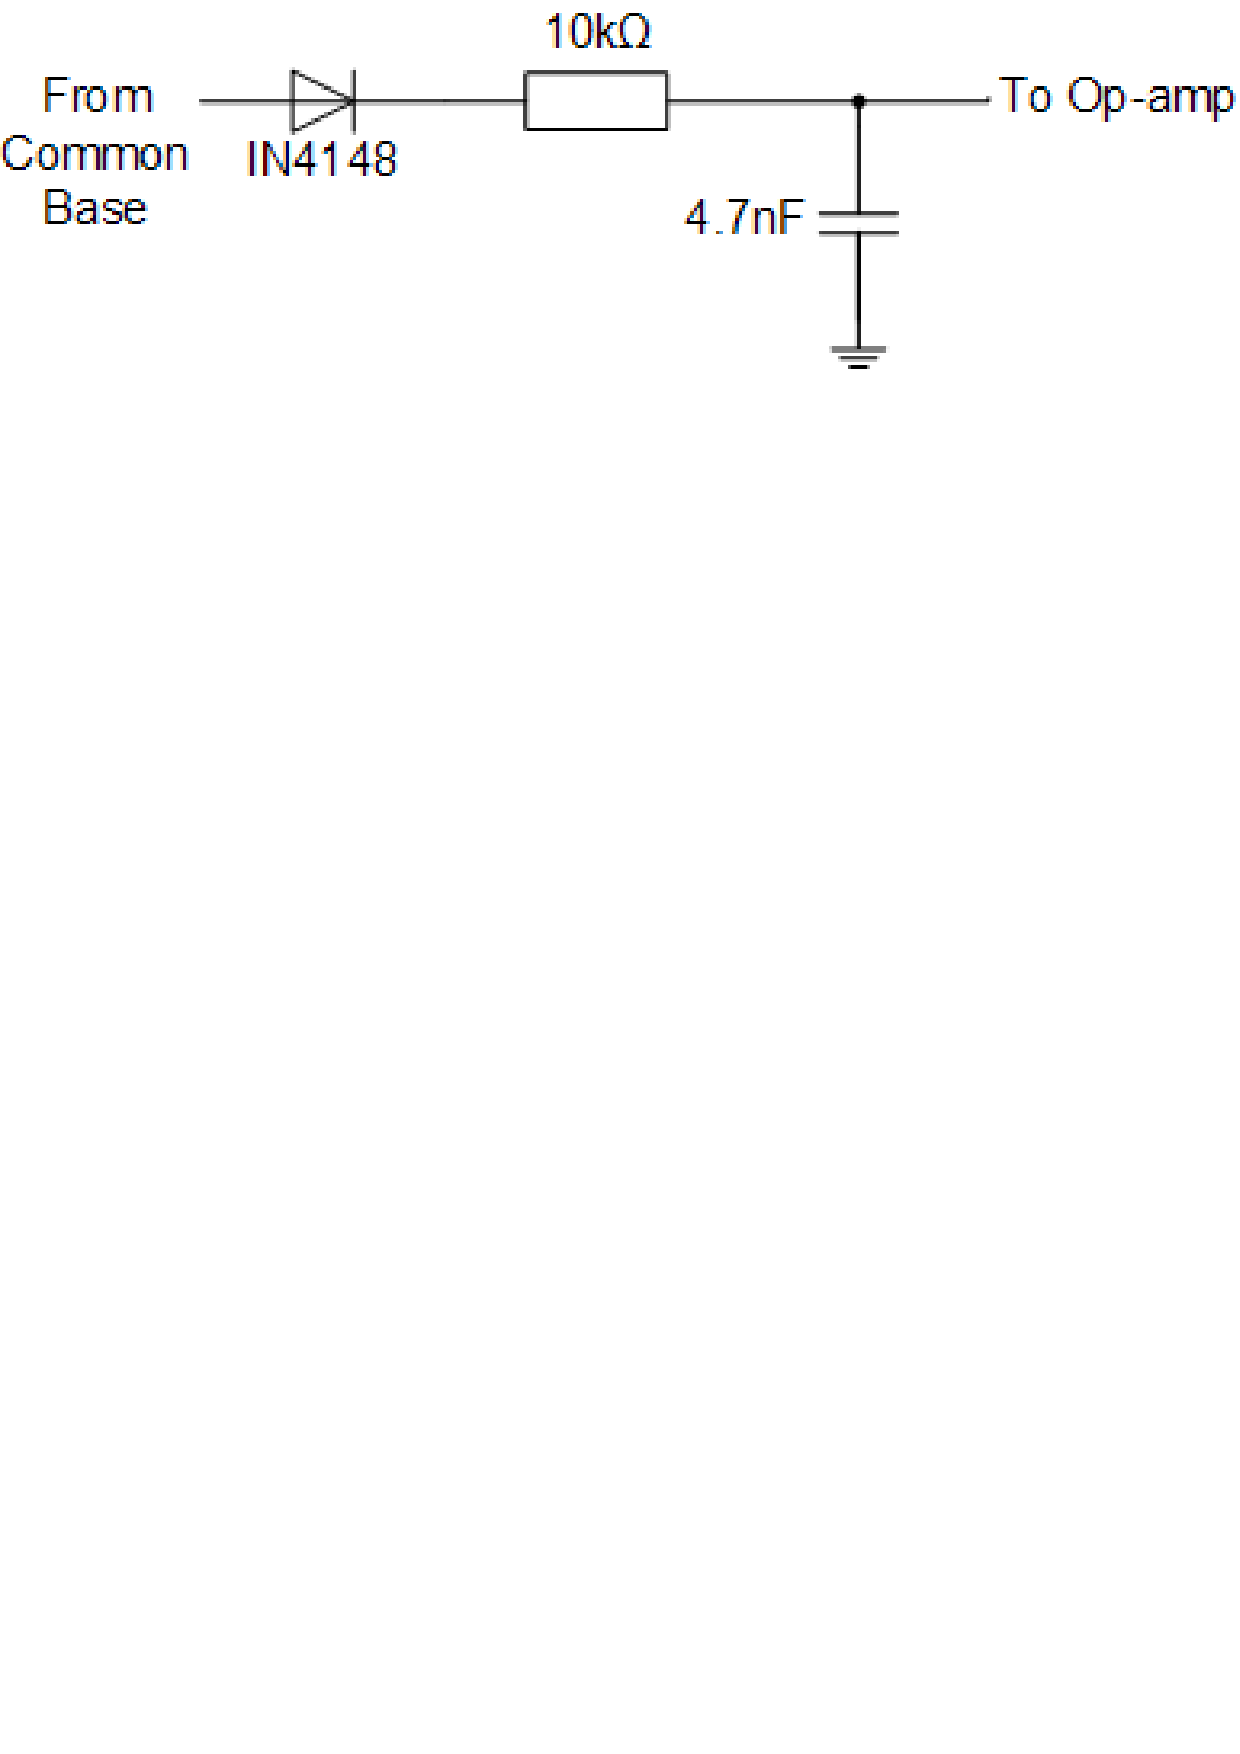
\includegraphics[scale=0.7]{Rectifier}
  \caption{Rectifier and Low-Pass Filter Configuration}
\end{figure}

The voice signal was then amplified by an Op amp.  This was to have a
gain of about 10, a high $Z_{in}$ and a medium $Z_{out}$.  The op-amp
was biased in such a way to try to achieve all these.  It is a very
simple configuration that is very similar to one used in the lab
experiments.  Even though the 741 is an inferior product it was used
because it is cheap and the application it is needed for is not
`mission-critical'.  The last resistor (that goes to ground) can be
replaced with a variable resistor.  This will affect the amount of
gain of the Op-amp and thus can be used as a volume control.  \\ The
configuration is shown below.

\begin{figure}[htb]
  \centering
  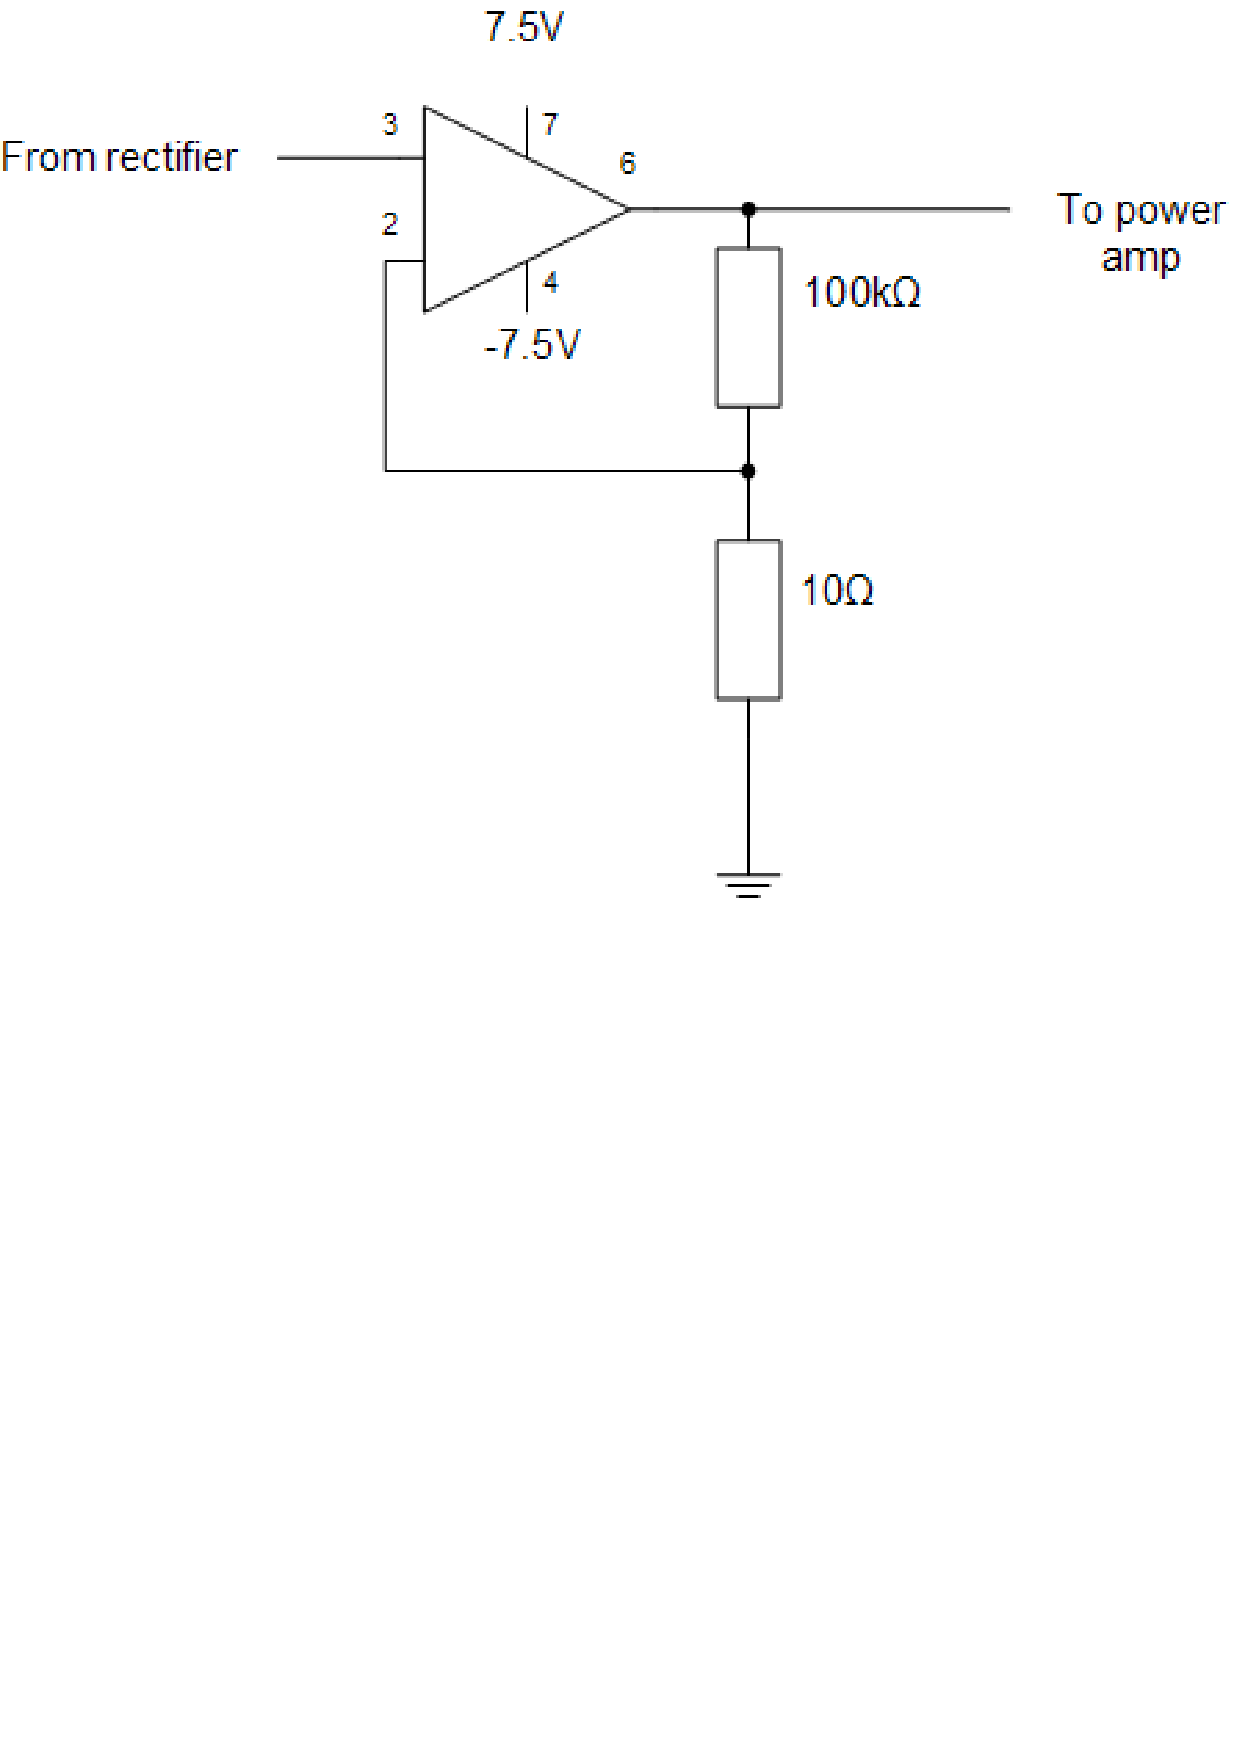
\includegraphics[scale=0.7]{Op-amp}
  \caption{Operational Amplifier Configuration}
\end{figure}

The last stage of the radio is to give the signal the power it needs
to drive the speaker.  As the output impedance of the Op-amp is quite
high, not much much current flows.  This means that it can't drive the
speaker directly.  Thus a power amplifier is needed to increase the
current.  I chose a Class AB amplifier because it has less cross-over
distortion and is much more efficient than a Class A amplifier.  In
Class AB amplifiers, the two transistors to be on at the same time,
which means that the non-linear nature of the Class B amplifier is
effectively eliminated.  The Class AB configuration takes the good
parts of Class A and B, so it is the natural choice for audio
applications.  The configuration is shown below.

\begin{figure}[h]
  \centering
  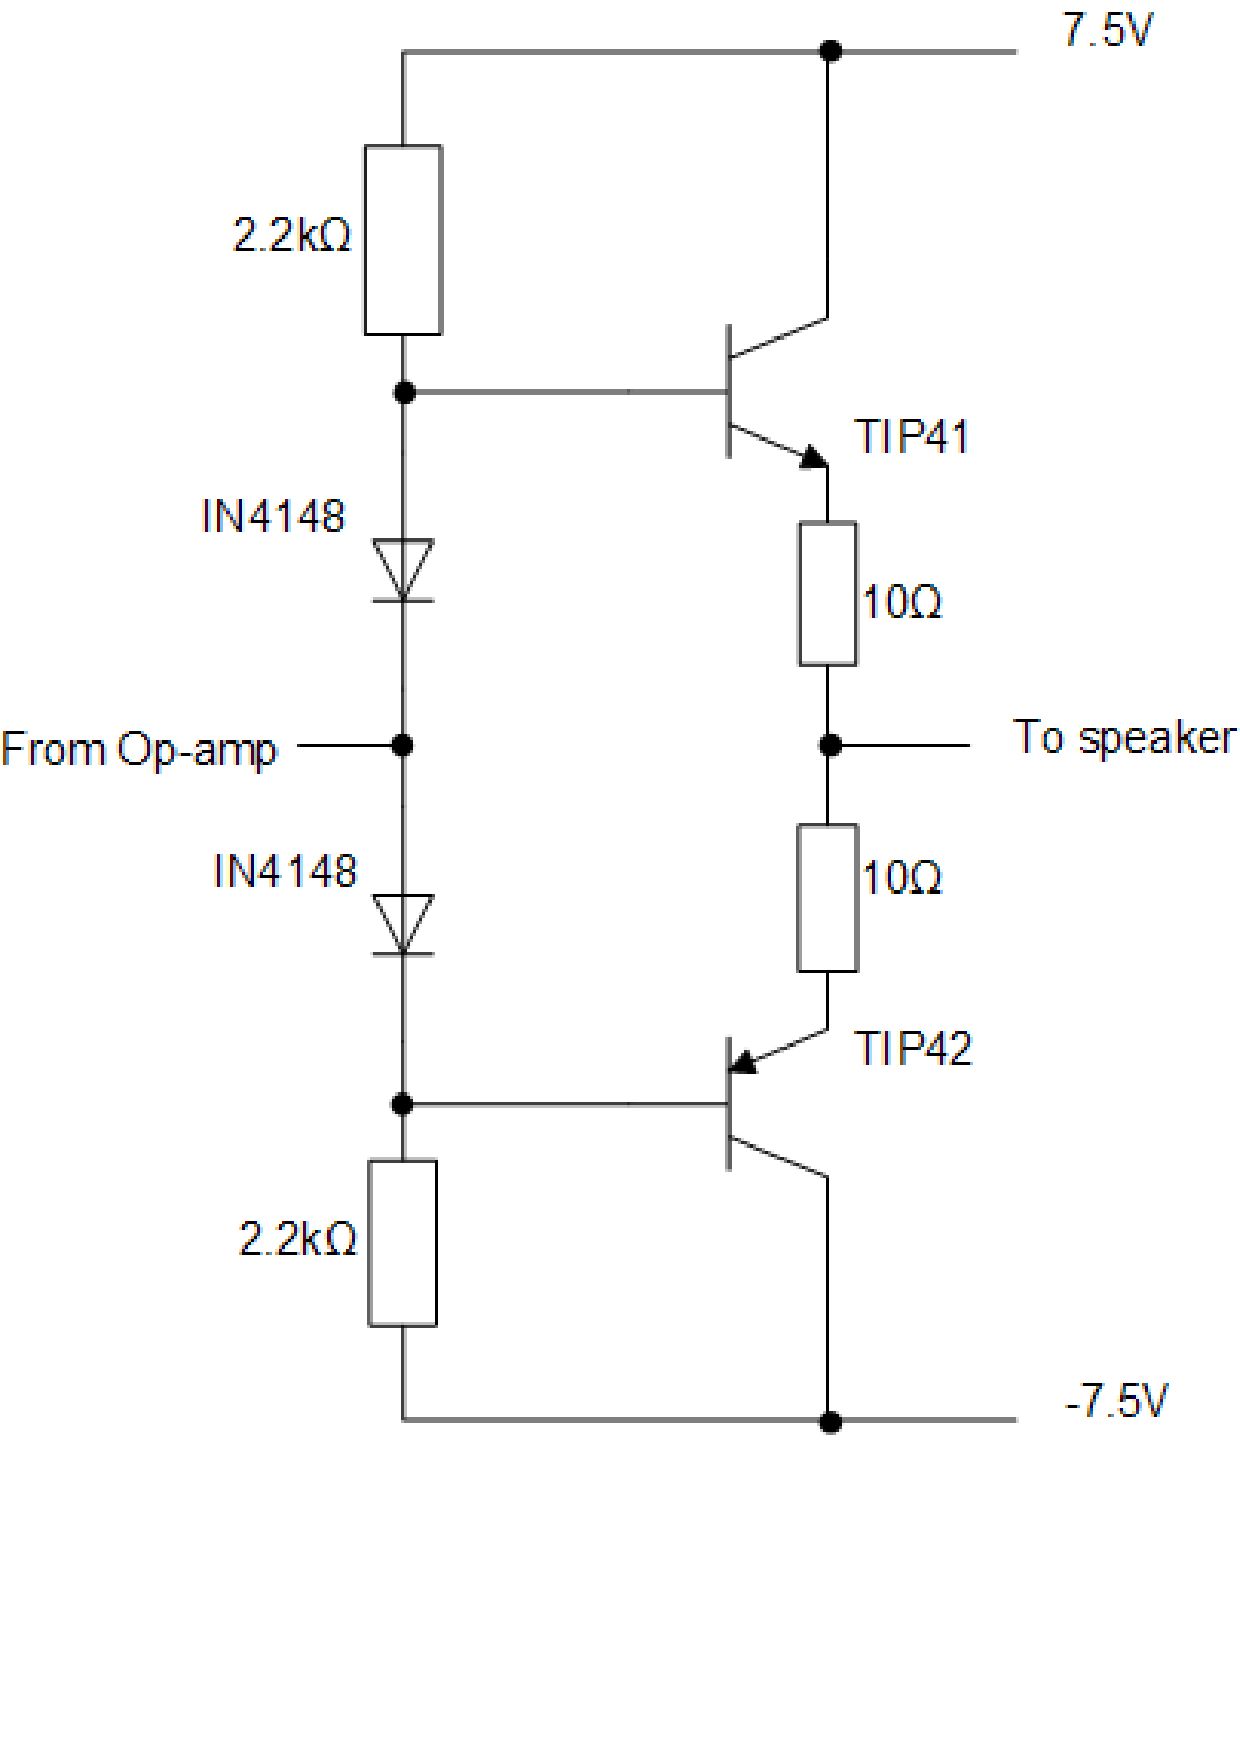
\includegraphics[scale=0.7]{Power-amp}
  \caption{Power Amplifier Configuration}
\end{figure}
\pagebreak

\chapter{Performance, Problems and Improvements}
The the biggest problem is that the radio doesn't actually work.  This
could be caused by many things, but I suspect that it is caused by the
impedance not being matched between the Op-amp and the power
amplifier.  With the oscilloscope (and the help of Peter Coard), I can
see that there is an RF signal at the output, but it is very noisy.
This is probably caused by the impedance between stages not matching.
I have tried to modify the input and output impedances, but to no
avail.

Each component is working correctly in isolation.  The gain of the
emitter follower is almost exactly one, and as shown in the appendices
the output impedance is $440\Omega$.  This is quite low, meaning that
the output current is quite high.  The common base amplifier also
seems to be doing it's job correctly.  When a sinusoidal wave of a few
tens of millivolts is fed into the emitter follower, the output of the
common base is about a few millivolts, thus giving an amplification of
a about a thousand.  The output at this stage is almost a perfect sine
wave.  The input impedance was discovered to be $800\Omega$ and the 
output impedance was $9k\Omega$.

The signal then passes through a diode and a low-pass filter.  At the
output of the diode, only the positive component is then filtered.
The time constant was set by the product of the capacitance and
resistance of the circuit.  This part also seems to work correctly in
isolation.

The op-amp was tested and found to have a gain of about 10.  The input
impedance is and the output impedance is.  When a signal from the
signal generator is applied, the output is approximately ten times
larger, and is a true sign wave with no distortion.

The power amp increases the current so as to drive the speakers.  This
was tested by measuring the current flowing into and out of the
amplifier.  The input impedance was found to be $9\Omega$, and the 
output impedance was $318\Omega$.  The voltage gain of the device was
approximately one.  The very low input impedance could also attribute
to the radio not working.  This means that is was drawing too much current 
from the Op-amp stage.  The output impedance however was at a quite
an acceptable level.

One improvement that could be made is the inclusion of a variable
resistor to work as a volume control.  This would involve replacing
the $10\Omega$ resistor with a $10\Omega$ `turn-pot' resistor.  This
would modify the gain, thus modify the speaker volume.

\chapter{Cost Estimate}
This is a rough estimate of the cost of resources and time.  It is assumed
it would be made on a printed circuit board with a case.
\begin{itemize}
	\item IC's \times 3 = $6
	\item Capacitors \times 4 = $2
	\item Power transistors \times 4 = $2
	\item PCB \times 1 = $200
	\item Case \times 1 = $100
	\item Labour $40/hr \times 18 = $720 \\ \\\
	\large \textbf{Grand Total: \$1030}
\end{itemize}

\pagebreak
\chapter{Appendices}

\section{Biasing the Emitter Follower}
\subsection{Calculate $V_{E}$}
\begin{eqnarray*}
  V_{E} & = & \frac{1}{2} \times V_{CC} \\
  {} & = & \frac{1}{2} \times 7.5V \\
  {} & = & 3.75V
\end{eqnarray*}

\subsection{Choose $R_{E}$}
\[V_{E} = 7.5k\Omega\]

\subsection{Calculate $R_{1}$ and $R_{2}$}
\begin{eqnarray*}
  V_{B} & = & V_{E} + 0.7V \\
  {} & = & 4.35V
  \end{eqnarray*}
  So, the ratio of $R_{1}$ to  $R_{2}$ is 1:1.17 \\
  $\therefore\, \ R_{1} = 120k\Omega$ and $R_{2} = 150k\Omega$

\subsection{Choose $C_{c1}$ and $C_{C2}$}
\begin{eqnarray*}
  C_{C1} & = & 0.1 \mu F \\
  C_{C2} & = & 0.1 \mu F 
\end{eqnarray*}

\subsection{Calculate $ Z_{in}$ and $ Z_{out}$}
\begin{eqnarray*}
  Z_{out} & = &\frac{{R_{out} // {R_{E} + R_{in}}}}{{\beta + 1}} \\
\end{eqnarray*}

\begin{eqnarray*}
  V_{E} & = &  7.5 - 0.7 \\
  & = & 6.8V \\
\end{eqnarray*}

\begin{eqnarray*}
  I_{E} & = & \frac{6.8V}{7.5k\Omega} \\
  & \approx & 9mA \\ 
\end{eqnarray*}

\begin{eqnarray*}
  R_{o} & = & \frac{V_{A}}{I_{C}} \\ 
  & = & \frac{3.75V}{9mA} \\
  & = & 416\Omega \\
\end{eqnarray*}

\begin{eqnarray*}
  R_{o} & = & \frac{V_{BE}}{I_{E}} \\ 
  & = & \frac{0.7}{9mA} \\
  & = & 77.8\Omega \\
\end{eqnarray*}

\begin{eqnarray*}
  \frac{R_{in}}{{\beta + 1}} & = & 13k\Omega \\ 
  & = & \frac{13k\Omega}{406+1} \\
  & = & 31.9\Omega \\
\end{eqnarray*}

\begin{eqnarray*}
  \therefore\,\  R_{out} & = & 416 // (77.8+31.9) \\
  & = & 416 // \frac{1}{\frac{1}{77.8} + \frac{1}{31.9}} \\
  & = & 440\Omega \\
\end{eqnarray*}

As the input resistance is simply the two input resistors in series,
\begin{eqnarray*}
  R_{in} & = & 150k\Omega + 120k\Omega \\
  & = & 270k\Omega
\end{eqnarray*}

\section{Biasing the Common Base}
\subsection{Calculate $R_{E}$}
We want $I_{C} \approx 0.5mA$
\begin{eqnarray*}
  \therefore R_{E} & = & \frac{V_{CC} + V_{CE}}{I_{C}} \\
  & = & \frac{7.5V + 0.6V}{0.5mA} \\
  & = & \frac{6.9V}{0.5mA} \\
  & = & 14k\Omega
\end{eqnarray*} \\

\subsection{Calculate $R_{C}$}
We also want $V_{o} \approx 3V$
\begin{eqnarray*}
  \therefore R_{C} & = & \frac{V_{CC} - V_{o}}{I_{C}} \\
  & = & \frac{7.5V - 3V}{0.5mA} \\
  & = & \frac{4.5V}{0.5mA} \\
  & = & 9k\Omega
\end{eqnarray*}

\section{Rectifier}
The rectifier circuit forms an RC circuit with time constant $\tau$ =
RC. This time must be short compared to the period of AM radio
frequency band (500kHz to 1.6MHz), but long compared to human speech
(20Hz to 20kHz).\\

\noindent Thus:  \\
AM Radio: 500kHz to 1.6MHz \\
Period: $2\mu$s to $0.67\mu$s \\

\noindent Human Speech: 20Hz to 20kHz  \\
Period: $50$ms to $50\mu$s\\

$\therefore$ we want:
\begin{eqnarray*}
\tau & = & R \times C \\
  & = & 1k\Omega \times 4.7nF \\
  & \approx & 5ms
\end{eqnarray*}\\
Gives a time between the ranges, and a frequency of about 200kHz.

\pagebreak
\section{Full circuit diagram}

\begin{figure}[b]
  \centering
  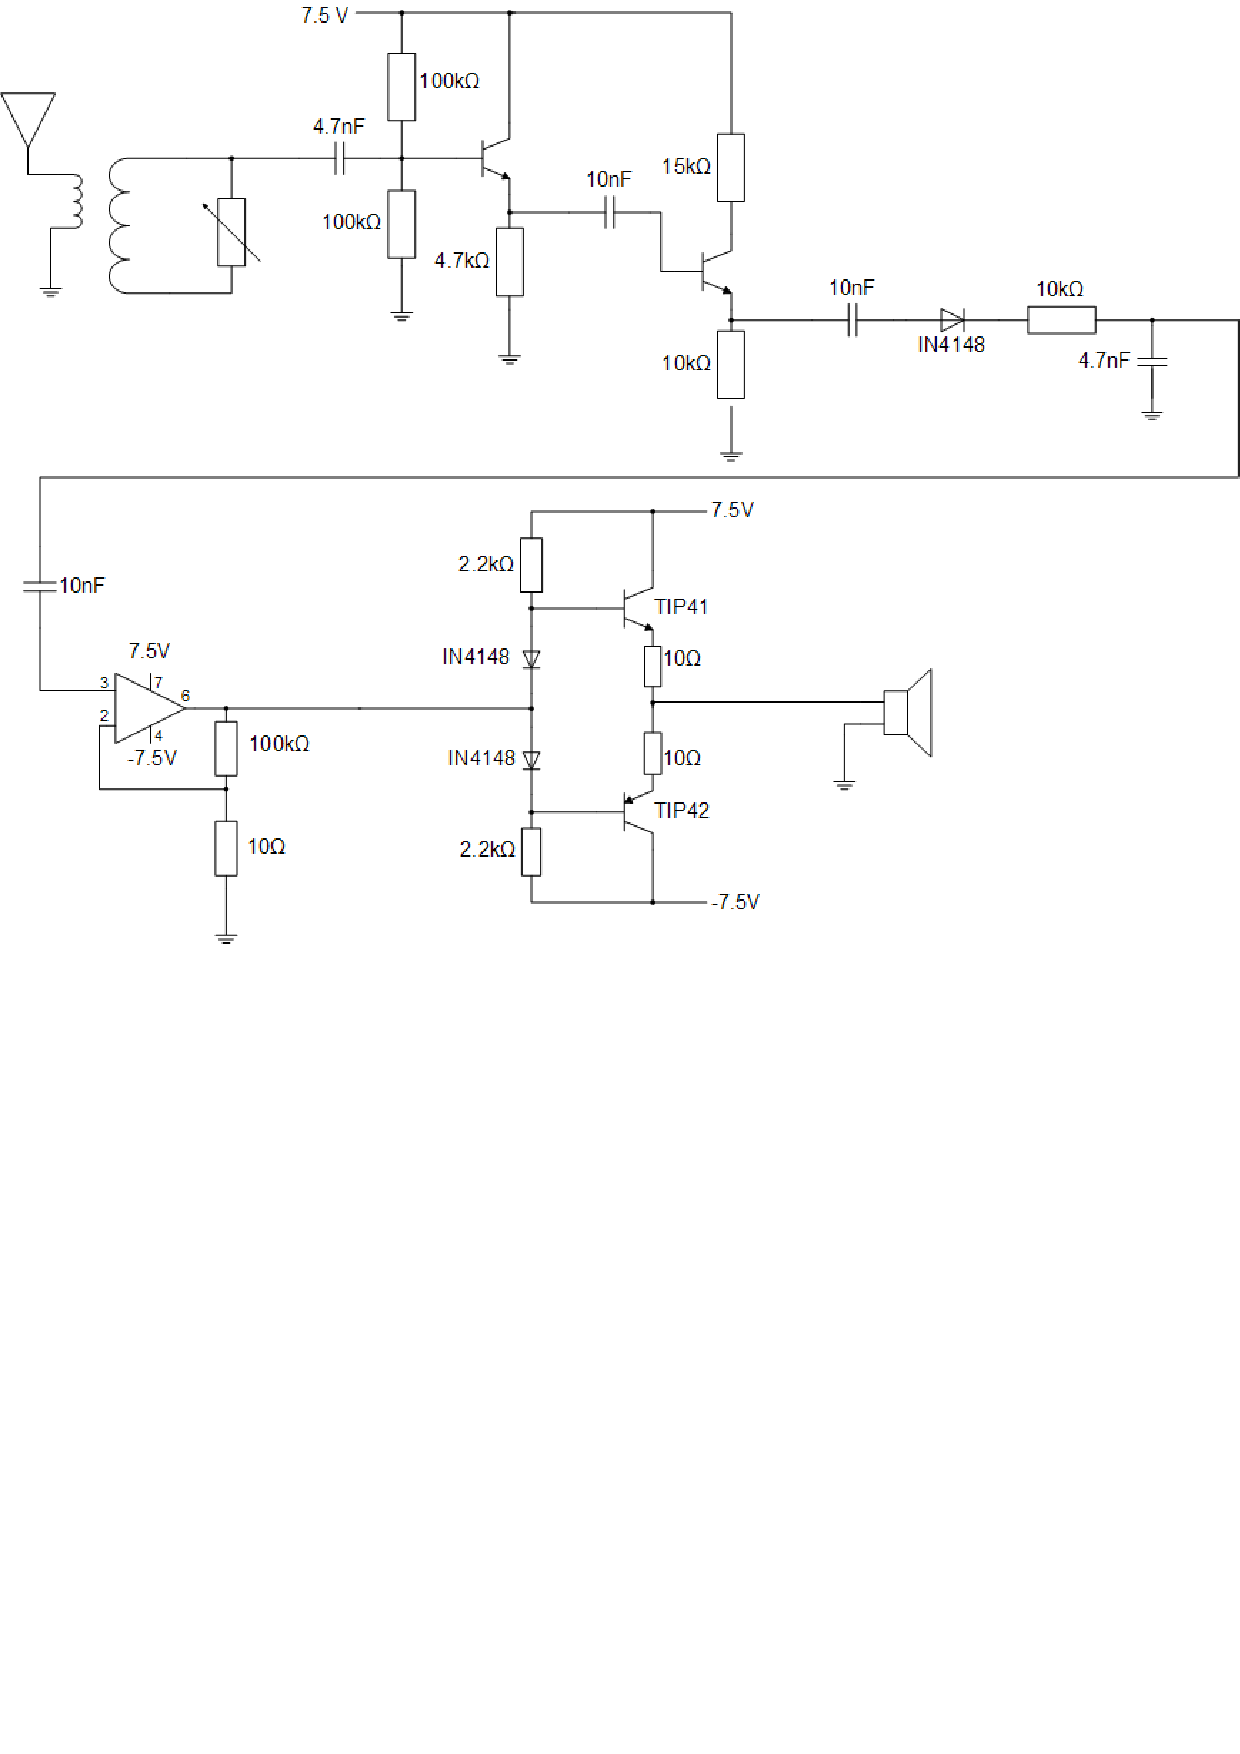
\includegraphics[scale=0.6, angle=90]{Circuit-diagram}
  \caption{Full Circuit Diagram of the radio}
\end{figure}

\end{document}